%%%%%%%%%%%%%%%%%%%%%%%%%%%%%%%%%%%%%%%%%%%%%%%%%%%%%%%
%%%%%%%%%%%%%%%%%%%%%%%%%%%%%%%%%%%%%%%%%%%%%%%%%%%%%%%

% The High-Granularity Calorimeter and HGCROC

% Description of the HL-LHC phase
% What are the main changes in the CMS detector that are expected for the HL-LHC?
% Description of the High-Granularity Calorimeter
% The read-out structure and HGCROC
% Description of HGCROC
% How can you characterize the chip?
% The irradiation test: TID and SEE
% Improvements in the chip design
% Conclusion

%%%%%%%%%%%%%%%%%%%%%%%%%%%%%%%%%%%%%%%%%%%%%%%%%%%%%%%
%%%%%%%%%%%%%%%%%%%%%%%%%%%%%%%%%%%%%%%%%%%%%%%%%%%%%%%

\chapter{The CMS Endcap Calorimeter Upgrade}

After nearly fifteen years of dedicated service, the LHC will undergo a major upgrade towards the High Luminosity LHC phase (HL-LHC), which is expecting to start its operations by the end of 2029.
The upgraded machine has been designed to operate at a  centre-of-mass energy of 14~TeV and to achieve a peak instantaneous luminosity of $L=5\cdot10^{34}\;cm^{-2}s^{-1}$: in these unprecedented running conditions, a remarkable integrated luminosity of 4000~$fb^{-1}$ is expected to be collected over the anticipated ten years of data-taking. 
With the HL-LHC upgrade, the amount of collected data will significantly increase, so as the potential for new discoveries at the LHC. The increased statistics will allow for more precise measurements of the SM properties but will also improve the potential for new discoveries, enhance the sensitivity to rare processes and possibly unveil the presence of previously unknown particles and BSM scenarios.

The higher luminosities of the HL-LHC will also result in exceedingly high pile-up rates, with $\mathcal{O}(200)$ events per bunch crossing and unprecedented radiation levels, with fluences of up to $3.5\times10^6\,\textrm{s}^{-1}\,\textrm{cm}^{-2}$ and a total absorbed dose of up to $\sim$$200\,\textrm{Mrad}$, thus posing several technical challenges for the operation of the detectors and the entire infrastructure.
In order to maintain its excellent physics performance in the high pile-up environment of the HL-LHC, the CMS Collaboration, as well as the other LHC experiments, is planning a series of major upgrades of the sub-detectors. The upgrade development and realization has already started during the Second Long Shutdown (LS2, 2018-2022) and will continue in the Third Long Shutdown (LS3, 2025-2029) when the installation and commissioning of the new detectors will be performed. 

In this chapter, after a brief overview of the CMS upgrade plans in Sec. {?}, the focus will be directed towards the High Granularity Calorimeter (HGCAL), that will replace the current endcap calorimeters and completely renovate the CMS forward calorimetry strategy. The HGCAL detector will provide the very first large-scale silicon-based imaging calorimeter employed in a high-energy physics experiment, with extremely fine transverse and longitudinal granularity, including a total of 6 million channels. Besides the unprecedented read-out segmentation, the performance requirements for the front-end electronics will be extremely stringent and calls for ad-hoc electronics development. With an excellent technical effort to meet all these requirements, the HGCROC3 is the final version of the ASIC specifically designed to readout the modules of the future HGCAL. 
The characteristics of the HGCROC will be described in Sec {?}, while Sec {?} will present the irradiation campaigns performed on the chip in order to prove its radiation hardness. 

\section{Upgrades of the CMS detector}

In the context of the future HL-LHC phase (Phase-2), the CMS detector upgrades programme has the main objective of maintaining the current physics performance under a new unprecedentedly complex environment. 
After years of operations, many current detector components have become inadequate to withstand high luminosity conditions and will either go through a complete replacement or a significant upgrade of already existing modules. There are three main points the CMS Collaboration has to consider to ensure that the detector's capabilities align with the ambitious research goals of the HL-LHC era:
\begin{itemize}
    \item [-] The unprecedented radiation doses will necessitate a complete replacement of the tracker and endcap calorimeter systems, the adoption of new technologies for the electromagnetic barrel (EB), and substantial enhancements to the electronics systems in the barrel calorimeters and muon detectors.
    \item [-] The increase in the pileup rate will require highly granular readouts wherever possible, the implementation of precision timing detectors, and innovative approaches to pileup mitigation.
    \item [-] The high luminosity will result in an increased data stream, highlighting the crucial need for substantial improvements to the L1 Trigger primitives and the overall Trigger and Data Acquisition System (TriDAS).
\end{itemize}

% Figure 3.1 illustrates a cross-section of the CMS detector, outlining the planned upgrades for the HL-LHC. The subdetectors within the green boxes will undergo complete replacement, while the purple boxes represent new detector systems, not part of the current CMS design, that will be integrated.

To enhance the detector's granularity and reconstruction performance while minimizing the material budget, the tracking system will be entirely replaced. This involves employing smaller pixel detectors for the inner tracking system and incorporating strips and macro pixel sensors for the outer tracking stations, extending coverage up to $|\eta|=3.8$. These changes are expected to improve longitudinal and transverse resolutions, as well as reduce fake rates, enabling the reconstruction of L1 trigger tracks up to $|\eta|=2.4$.

The endcap calorimeters will be replaced with the HGCAL, a high-granularity sampling calorimeter designed to enhance shower separation, particle identification, and provide precise timing information.

Additionally, to increase granularity and provide additional timing measurements, upgrades to the ECAL and HCAL barrel electronic readout systems are planned. The redundancy of the current muon detection system, comprising DTs, RPCs, and CSCs, will be augmented by the installation of Gas Electron Multiplier chambers and a new generation of RPCs. These enhancements will extend coverage up to $|\eta|=2.8$ and $|\eta|=2.4$, respectively.

Furthermore, Multiple MIP timing detectors (MTD) will be positioned in front of the barrel and endcap calorimeters. This additional layer will improve the timing information on charged candidates, which is crucial for disentangling the approximately 200~PU interactions foreseen per bunch crossing.

Finally, the trigger and data acquisition systems will be completely replaced, redesigning the Level-1 hardware trigger to include tracking and high-granularity calorimeter information exploited via the extensive use of state-of-the-art FPGAs and ML techniques.

A schematic overview of the CMS Phase-2 upgrade is depicted in Figure \ref{fig:CMSUpgrade}. 
% In this illustration, the green boxes represent the upgraded systems pertinent to the discussion in this chapter. Conversely, the orange boxes denote upgrades that fall outside the scope of this thesis.

\begin{figure}
    \centering
    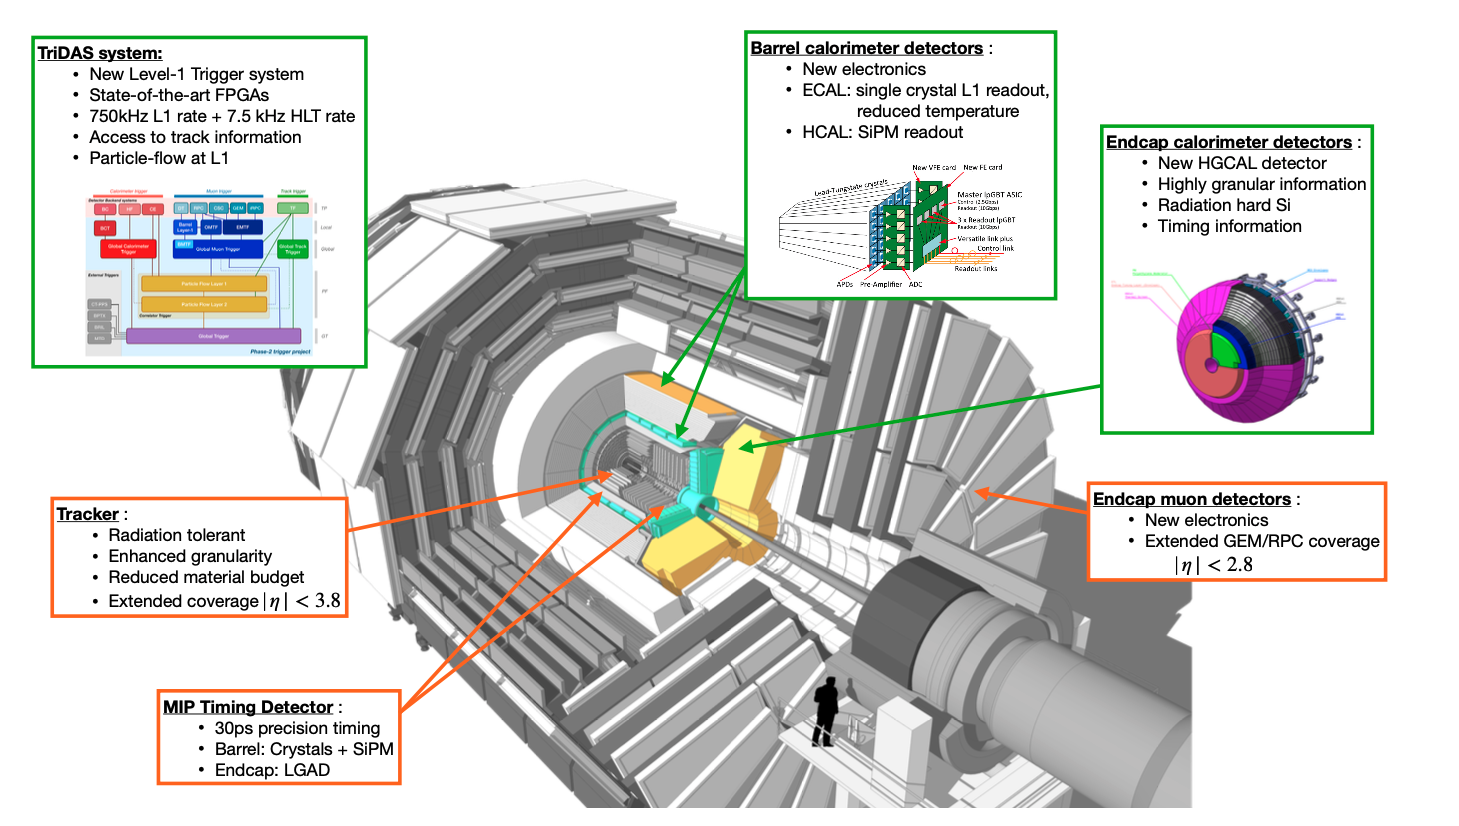
\includegraphics[width=0.75\linewidth]{Figures//HGCAL/Screenshot 2024-03-19 at 15.32.21.png}
    \caption{Enter Caption}
    \label{fig:CMSUpgrade}
\end{figure}

\section{The High-Granularity Calorimeter design}

Among the CMS detector updates, one of the most ambitious projects is the High Granularity Calorimeter (HGCAL), a high-granularity sampling calorimeter designed to replace the existing CMS endcap calorimeter in order to to maintain a excellent physics performance under the high pile~up and harsh radiation environment of HL-LHC.

The existing forward calorimeters, the $\textnormal{PbWO}_4$-based electromagnetic calorimeter (EE) and the plastic scintillator based hadron calorimeter (HE), were initially designed to withstand a total integrated luminosity of 500 $\textnormal{fb}^{-1}$. 
The performance degradation much beyond this integrated luminosity leads to an unacceptable loss of physics performance.
The High Granularity Calorimeter (HGCAL) is probably one of the most abitious projects.\cite{TDR} will replace the existing CMS endcap calorimeter to maintain a excellent physics performance under the high pile~up and harsh radiation environment of HL-LHC.
The HGCAL detector will consist of hexagonal silicon-based modules for the electromagnetic and part of the hadronic section, and of plastic scintillator tiles with SiPM read-out for the remaining low-radiation hadronic section.
With this ambitious project, the CMS forward calorimetry will be provided with an extremely fine transverse and longitudinal granularity, including a total of 6~million channels.
Besides the unprecedented readout segmentation, the performance requirements for the front-end electronics are extremely stringent: dynamic range over 16 bits equivalent ($0–10\,\textrm{pC}$), noise below 2500~electrons, high-precision timing information ($25\,\textrm{ps}$) in order to mitigate the pileup effect, low power consumption ($\sim$$15\,\textrm{mW/channel}$), and low temperature operation ($240\,\textrm{K}$).

With an excellent technical effort to meet all these requirements, the HGCROC3 is the final version of the ASIC specifically designed to readout the modules of the future HGCAL. 
During my thesis project, I conducted an extensive characterization of the HGCROC3 chip, with particular emphasis in testing its performance both under normal conditions and radiation environments.
This section contains a general overview of the architecture of the chip and its operation, a description of the main radiation effects, the testing procedures and the results from the irradiation campaigns.
